\section{Experiments}
\label{sec:experiments}
% 実験の目的
The experiments were designed to evaluate the performance of our proposed method on real-world datasets, focusing on two key aspects: (1) the accuracy of dense pattern identification and (2) the accuracy of dense interval detection. To achieve this, we compare our approach with existing methods by introducing two novel evaluation metrics.
% 共通して用いるデータセットの説明
The datasets used in the experiments are publicly available and are often utilized as benchmarks in pattern mining research\cite{fournier2016spmf}. 

\begin{table}[t]
    \centering
    \begin{threeparttable}
    \caption{Statistical information of real-world datasets}
    \label{tab:dataset_stats}
    \begin{tabular}{|c|c|c|}
    \hline
    Dataset       & No. of transactions & No. of unique items \\
    \hline
    Retail        & 88,162              & 16,470               \\
    OnlineRetail  & 541,909*            & 4,070                \\
    Kosarak       & 990,002             & 41,270               \\
    ChicagoCrime  & 1,000,000           & 42,655               \\
    \hline
    \end{tabular}
    \begin{tablenotes}
        \small{\item *Deleted blank transactions in preprocessing}
    \end{tablenotes}
    \end{threeparttable}
\end{table}


\subsection{Experiment 1: Dense Pattern Identification}
% 尺度の導入
\subsubsection{Metrics}
To assess the accuracy of pattern identification, we use F1-score metrics the same as in the preliminary experiments.

% 正解データの用意
To compute the above metrics, we generate ground truth patterns for each dataset. For the Retail dataset, the ground truth is defined as the dense patterns that satisfy a $minL$ of 500 and a $minsup$ of 10\%. For the remaining datasets, the ground truth patterns are those meeting a $minL$ of 250 and a $minsup$ of 10\%. This ground truth is obtained using an extended version of the Apriori algorithm, an exact solution method that precisely extracts the patterns satisfying these conditions.

\subsubsection{Methods}
% 比較手法の紹介
We compare Plant Model (Global Suppression) to five baseline methods: Apriori\cite{agrawal1994fast}, PFPM\cite{tanbeer2009discovering}, PPFPM\cite{kiran2017discovering}, LPFIM\cite{mahanta2005finding}, and LPPM\cite{fournier2021mining}.
Apriori extracts itemsets that appear frequently in the entire data set. PFPM and PPFPM extract itemsets that appear periodically. Specifically, the former method extracts itemsets that are periodic across the entire data set, while the latter method relaxes the conditions to extract patterns that show periodicity in some parts of the data.
LPFIM and LPPM are methods for extracting both periodic itemsets and intervals that exhibit periodicity.


% パラメータの探索
\subsubsection{Parameters}
We perform a grid search per dataset to select both the baseline methods’ parameters and the Plant Model’s hyperparameters. For the baselines, we simply take the configuration that achieves the highest score within the search space. In principle, if the Plant Model is allowed unlimited computational cost, it will almost certainly generate agents matching every dense pattern—driving its F1‐score to 1. Therefore, in this experiment we choose hyperparameters that balance extraction accuracy against execution time. The search spaces and the specific parameter values used in the experiments for all methods are detailed in Appendix \ref{sec:params_space} and \ref{sec:params}.

% The same grid‐search procedure used in Experiment 1 for Plant Model (Global Suppression) was also applied to Plant Model (Interval‐Restricted Suppression), tuning its settings to balance the Jaccard score and runtime.

\subsubsection{Experimental Conditions}
All baseline methods are deterministic algorithms and thus each was run only once. Because Plant Model (Global Suppression) is stochastic, we performed 20 independent trials and report the mean F1‐score. 

\subsubsection{Results of Experiment 1}
\begin{table*}[t]
  \centering
  \begin{threeparttable}
    \caption{Pattern identification F1‐scores for each method and dataset}
    \label{tab:f1_scores}
    \begin{tabular}{|c|cccc|}
      \hline
      Method & Retail & OnlineRetail & Kosarak & ChicagoCrime \\
      \hline
      Apriori                   & 0.017 & 0.003 & * & 0.006 \\
      PFPM                      & 0.529 & 0.220 & 0.933      & 0.614 \\
      PPFPM                     & 0.863 & 0.573 & 0.933      & 0.740 \\
      LPFIM                     & 0.964 & 0.872 & 0.966      & 0.952 \\
      LPPM                      & 0.967 & 0.832 & \textbf{0.983} & \textbf{0.976} \\
      Plant Model (Global Suppression)          & \textbf{0.990} $\pm$ 0.008 & \textbf{0.980} $\pm$ 0.012& 0.955 $\pm$ 0.030 & 0.974 $\pm$ 0.013\\
      \hline
    \end{tabular}
    \begin{tablenotes}
      \footnotesize
      \item[*] Apriori was terminated after running for approximately one week on the Kosarak dataset without producing any results, so no score was recorded.
    \end{tablenotes}
  \end{threeparttable}
\end{table*}

Table \ref{tab:f1_scores} shows that among the deterministic baselines, LPPM achieves the highest F1-score on Kosarak (0.983) and ChicagoCrime (0.976), with LPFIM slightly behind. PFPM and PPFPM deliver moderate performance, while Apriori fails to complete on Kosarak. Plant Model (Global Suppression) surpasses all baselines on Retail and OnlineRetail—reaching 0.990 $\pm$ 0.008 and 0.980 $\pm$ 0.012, respectively—and remains highly competitive on ChicagoCrime (0.974 $\pm$ 0.013). Although its score on Kosarak (0.955 $\pm$ 0.030) falls short of LPPM’s, Plant Model exhibits overall consistency across datasets and its ability to maintain top‑tier accuracy.
In particular, Plant Model (Global Suppression) was significantly more accurate for Retail and OnlineRetail ($p<0.01$).
This accuracy gain stems from its robustness to variable occurrence intervals. Table \ref{tab:dataset_std} quantifies this variability per dataset by averaging the standard deviation of each item set’s densest (least variable) interval—since those intervals drive dense‑pattern extraction—and shows that OnlineRetail’s variability is roughly three times higher than the others.
Conventional methods must raise the maximum‑interval threshold to cover diverse gaps, which lowers detected‑interval density and causes false positives and misses (as our preliminary experiments confirm). In contrast, the Plant Model’s sliding‑window evaluation needs no such threshold, so density remains constant despite interval variability, yielding stable, high‑precision extraction.



\begin{table}[t]
    \centering
    \caption{Variation in occurrence intervals for each dataset}
    \begin{tabular}{|c|c|}
        \hline
        Dataset & 
        \begin{tabular}{c}
            \scriptsize{Mean of minimum standard deviations} \\ 
            \scriptsize{of occurrence intervals}
        \end{tabular} \\\hline
        Retail & 7.31 \\
        OnlineRetail & 20.51 \\
        Kosarak & 6.12 \\
        ChicagoCrime & 6.95 \\
        \hline
    \end{tabular}
    \label{tab:dataset_std}
\end{table}

\begin{table}[t]
    \centering
    \caption{Average number of occurrences of top 20 items in each dataset}
    \begin{tabular}{|c|c|}
        \hline
        Dataset & Average occurrences of top 20 items \\ \hline
        Retail         & 8,917.25   \\
        OnlineRetail   & 29,706.70  \\
        Kosarak        & 120,358.25 \\
        ChicagoCrime  & 237,506.85 \\ \hline
    \end{tabular}
    \label{tab:itemcount}
\end{table}


% \subsubsection{Discussion.}

\subsection{Experiment 2: Dense Interval Detection}
\subsubsection{Metrics}
For dense interval detection accuracy, the similarity between the ideal dense intervals and those detected by the method is evaluated using the Jaccard coefficient defined in Equation (\ref{eq:Jaccard}). For a given itemset \(X\), let \(A\) denote the set of all timestamps within the ideal dense intervals and \(B\) denote the set of all timestamps within the dense intervals detected by the method.

\begin{IEEEeqnarray}{rCl}
J_X(A,B) & = & \frac{\lvert A\cap B\rvert}{\lvert A\cup B\rvert}\,. 
\label{eq:Jaccard}
\end{IEEEeqnarray}

The overall dense interval detection performance is then assessed by computing the mean Jaccard coefficient over all true dense patterns, where a value closer to 1 indicates higher accuracy. Ground‑truth dense sections are detected using the same method as in Experiment 1. Erroneous inclusion of non‑dense timestamps increases $\lvert A\cup B\rvert$. Omission of true dense timestamps decreases $\lvert A\cap B\rvert$. Both types of error lead to a reduced Jaccard coefficient. This clarifies how over‑ and under‑detection affect detection accuracy.


\subsubsection{Methods}
We compare the interval‑detection accuracy of two Plant Model variants—Plant Model (Global Suppression) and Plant Model (Interval‑Restricted Suppression)—against two baseline interval‑extraction methods, LPFIM and LPPM. LPFIM and LPPM serve as representative approaches for periodic interval detection. All methods use the same parameter settings as in Experiment 1.

\subsubsection{Parameters}
LPFIM, LPPM, and Plant Model (Global Suppression) use the same parameters as in Experiment 1.  
We applied the Experiment 1 grid search to Plant Model (Interval‑Restricted Suppression), selecting hyperparameters that balance F1-score and runtime.

\subsubsection{Experimental conditions}
As in Experiment 1, each baseline method was run once. Both Plant Model variants were run ten times, and the mean Jaccard coefficient across runs was used for comparison. 


\subsubsection{Results of Experiment 2}

\begin{table*}[t]
  \centering
  \caption{Jaccard coefficients for dense interval detection. }
  \label{tab:jaccard_scores}
  \begin{tabular}{|c|cccc|}
    \hline
    Method & Retail & OnlineRetail & Kosarak & ChicagoCrime \\
    \hline
    LPFIM                                    & 0.674 & 0.072 & 0.104 & 0.501 \\
    LPPM                                     & 0.811 & 0.213 & 0.324 & 0.545 \\
    Plant Model (Global Suppression)                        &  0.590 $\pm$ 0.032 & 0.738 $\pm$ 0.032& 0.090 $\pm$0.036 & 0.268 $\pm$ 0.026 \\
    Plant Model (Interval‑Restricted Suppression)                       & \textbf{0.984} $\pm$ 0.005& \textbf{0.987} $\pm$0.008& \textbf{0.621}$\pm$ 0.027& \textbf{0.867}$\pm$ 0.019\\
    \hline
  \end{tabular}
\end{table*}


\begin{figure*}[t]
  \centering
  %============ Retail ============%
  \begin{subfigure}[t]{\textwidth}
    \centering
    \begin{subfigure}[b]{0.48\textwidth}
      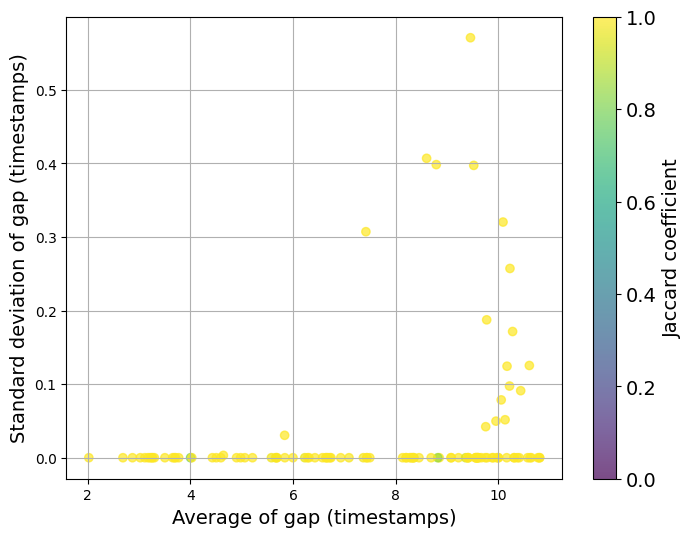
\includegraphics[width=\linewidth]{fig/retail_plant_plus_best_params.png}
      \caption{Plant Model (Interval‑Restricted Suppression)}
      \label{fig:retail_interval_restricted}
    \end{subfigure}
    \hfill
    \begin{subfigure}[b]{0.48\textwidth}
      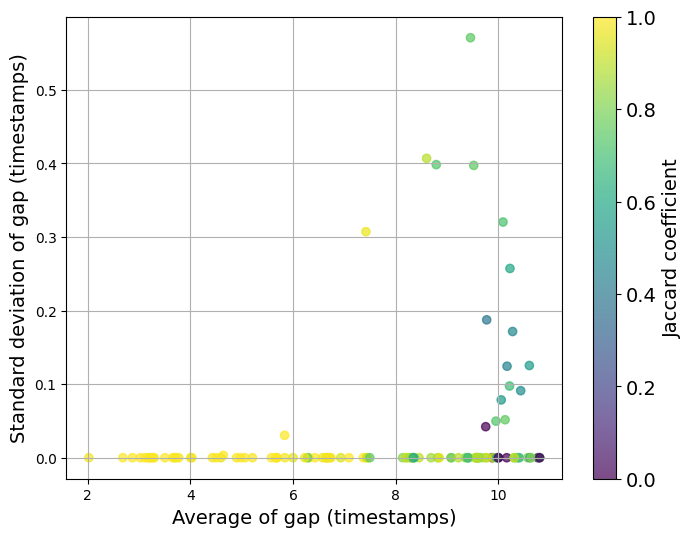
\includegraphics[width=\linewidth]{fig/retail_lppm_best_params.png}
      \caption{LPPM}
      \label{fig:retail_lppm}
    \end{subfigure}
    \label{fig:retail_jaccard}
  \end{subfigure}

  \caption{Jaccard coefficients for dense patterns in Retail. Each point represents an itemset: the x‑axis shows the mean occurrence gap, and the y‑axis shows the gap’s standard deviation. In this experiment, timestamps are recorded at fixed intervals. A coefficient closer to 1 denotes more accurate interval extraction.}
  \label{fig:jaccard_by_pattern}
\end{figure*}


Table~\ref{tab:jaccard_scores} highlights the limitations of periodic pattern mining methods: the Jaccard coefficients of LPFIM range from only 0.072 (OnlineRetail) to 0.674 (Retail), and although LPPM improves on these (0.213–0.811), it still misses or misdetects many of the true dense intervals. Plant Model (Global Suppression) falls even below these baselines because suppressing agent generation across all intervals prevents sufficient coverage. In contrast, the Plant Model (Interval-Restricted Suppression) shows better Jaccard coefficients than any other method because it keeps 
agents extracting candidates until nearly all dense intervals have been detected.

Fig. \ref{fig:jaccard_by_pattern} shows the Jaccard coefficient for each dense itemset in Retail dataset. LPPM achieves low interval detection accuracy for patterns with large average gaps and large gap variation, while the Plant Model (Interval-Restricted Suppression) maintains high Jaccard coefficients in exactly such difficult cases The results demonstrate that the Jaccard coefficient remains high even in such difficult cases. 


\subsection{Discussion}
% \begin{figure}[t]
%     \centering
%     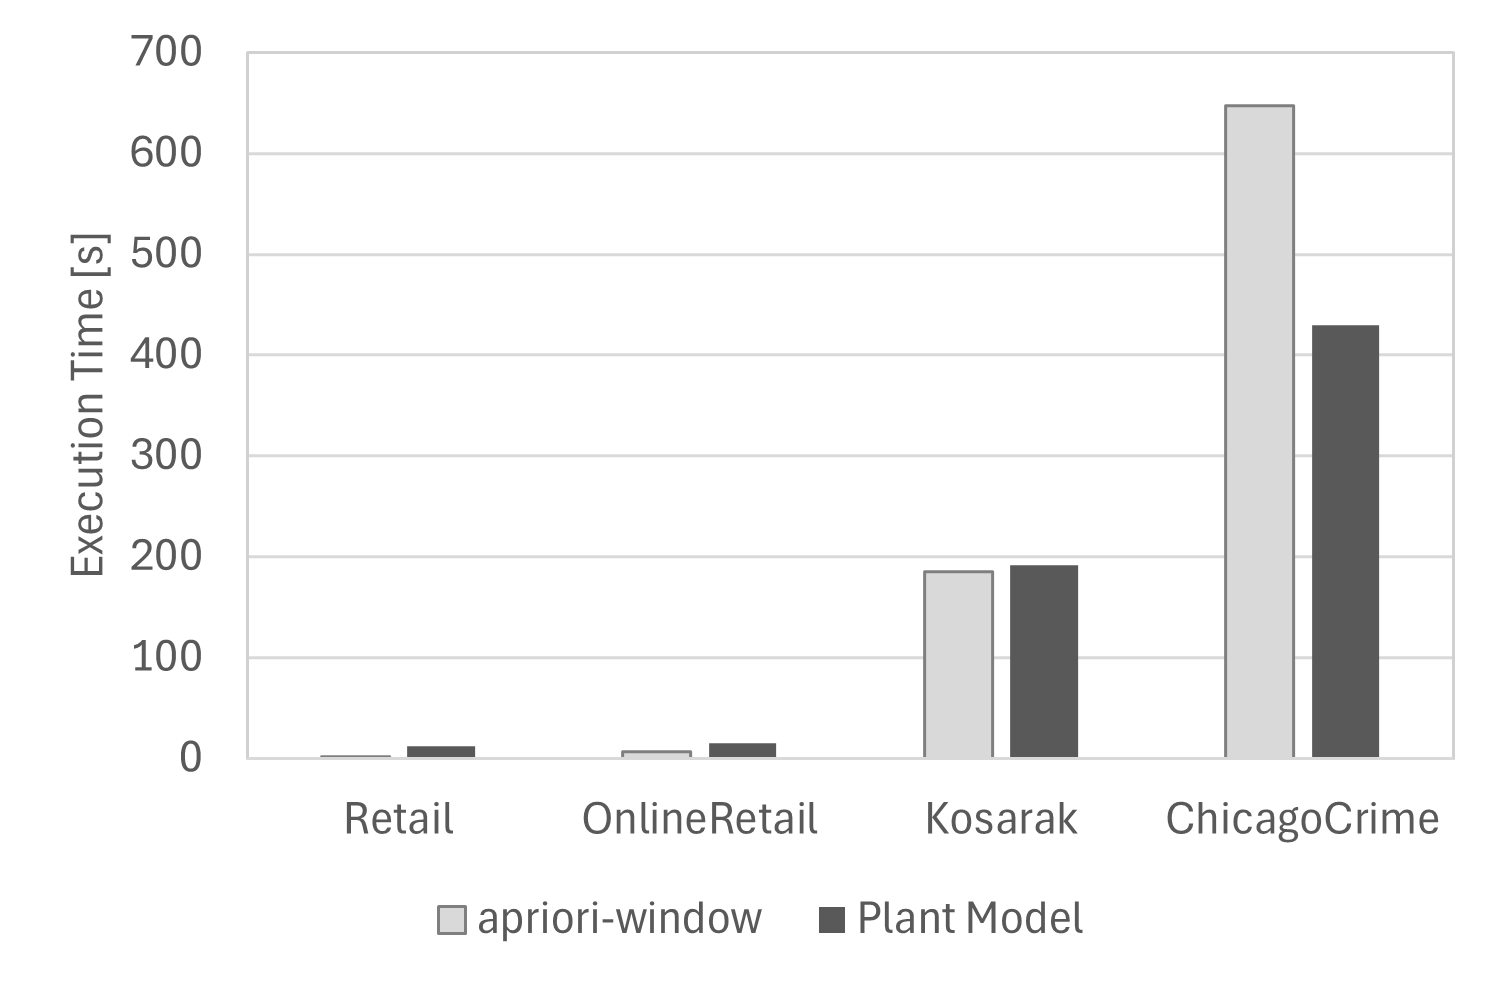
\includegraphics[width=1\linewidth]{fig/execution_time.png}
%     \caption{Execution time for Apriori‑window and both Plant Model variants.}
%     \label{fig:execution_time}
% \end{figure}

\begin{table*}[t]
\centering
\caption{Execution times (seconds) on various datasets}
\label{tab:exec-times}
\begin{tabular}{|c|cccc|}
\hline
\textbf{Method} & \textbf{Retail} & \textbf{OnlineRetail} & \textbf{Kosarak} & \textbf{ChicagoCrime} \\
\hline
Apriori-window & 1.62 & 6.63   & 185.73  & 647.53  \\
Plant Model (Global Suppression)           & 12.45  & 14.70  & 191.61  & 429.71  \\
Plant Model (Interval Restricted Suppression) & 138.68 & 114.22 & 3108.73 & 1433.24 \\
\hline
\end{tabular}
\end{table*}



We discuss the trade-off between accuracy and execution time for the proposed set of methods.
Table~\ref{tab:exec-times} compares execution times for Apriori‑window, Plant Model (Global Suppression), and Plant Model (Interval‑Restricted Suppression). 
All methods were implemented in Rust and executed on a Windows 11 Home 64‑bit PC with 32GB RAM and an AMD Ryzen 7 5700X (3.4GHz, 8cores/16threads).
For Retail and OnlineRetail, Apriori‑window remains fastest. On the larger Kosarak and ChicagoCrime datasets, Plant Model (Global Suppression) runs as fast as—or faster than—Apriori‑window.

As indicated by the execution time results in Experiment 1, Plant Model (Global Suppression) achieves a higher F1-score on ChicagoCrime with a shorter execution time than Apriori‑window, suggesting that its sampling strategy locates dense patterns very quickly. However, Experiment 2 shows that this variant attains lower interval‑detection accuracy than the baselines.

In contrast, Plant Model (Interval‑Restricted Suppression) delivers high Jaccard coefficients in Experiment 2, confirming precise extraction of dense intervals. Its execution times on the Retail, OnlineRetail, Kosarak, and ChicagoCrime datasets were 138.68s, 114.22s, 3108.73s, and 1433.24s, respectively, all exceeding those of both Apriori‑window and Plant Model (Global Suppression). Therefore, improving the time efficiency of this variant remains an important challenge.

